\usetikzlibrary{angles,quotes}
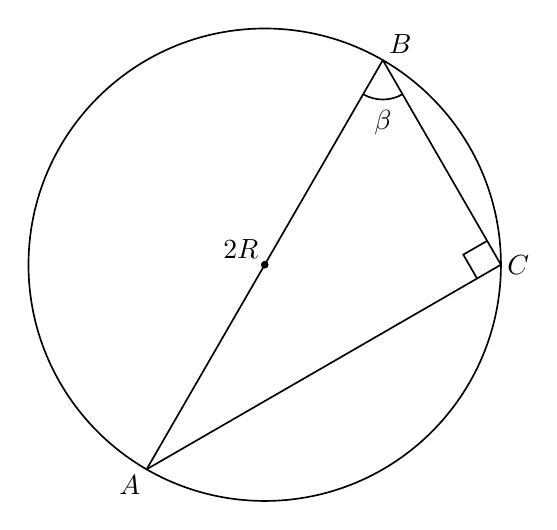
\begin{tikzpicture}[x=1cm,y=1cm,line width=.6pt,font=\normalsize]
\coordinate (O) at (0,0);
\coordinate (A) at (-1.5,-2.59808);
\coordinate (B) at (1.5,2.59808);
\coordinate (C) at (3,0);
\coordinate (R1) at (2.69690,-0.17500);
\coordinate (R2) at (2.52190,0.12810);
\coordinate (R3) at (2.82500,0.30310);
\draw (O) circle[radius=3cm];
\draw (A)--(B);
\draw (B)--(C)--(A);
\draw (R1)--(R2)--(R3);
\draw (B) ++(240:0.5cm) arc[start angle=240,end angle=300,radius=0.5cm];
\node[below left=2pt,inner sep=0pt] at (A) {$A$};
\node[above right=2pt,inner sep=0pt] at (B) {$B$};
\node[right=2pt,inner sep=0pt] at (C) {$C$};
\node at (1.5,1.80) {$\beta$};
\node[above left=2pt,inner sep=0pt] at (O) {$2R$};

% Explicit named circle-center points, painted after all region fills.
\fill (O) circle[radius=1.4pt];
\end{tikzpicture}
